\documentclass[11pt,oneside]{article}
\usepackage[utf8]{inputenc}
\usepackage[a4paper,top=2cm,left=2cm,right=2cm,bottom=2cm]{geometry}
\usepackage{import}
\usepackage[T1]{fontenc}
\usepackage[german,ngerman]{babel}
\usepackage[table]{xcolor}
\usepackage{amsthm, esvect}
\usepackage{mathtools}
\RequirePackage{amssymb, amsfonts, amsmath, latexsym, verbatim, xspace}
\usepackage{systeme}
\usepackage{multicol}
\usepackage{multirow}
\usepackage{framed}
\usepackage{array}
\usepackage{ragged2e}
\usepackage{graphicx}
\usepackage{pdflscape}
\usepackage{epstopdf}
\usepackage{booktabs}
\usepackage{pdfpages}
\usepackage{float} % Allows putting an [H] in \begin{figure} to specify the exact location of the figure
\usepackage{wrapfig} % Allows in-line images such as the example fish picture
\usepackage{tikz, graphicx} % tikz
\usepackage[position=top]{subfig}
\usepackage[bookmarks=true]{hyperref}%Links
\usepackage{enumerate}
\usepackage{enumitem}
\usepackage[german,ruled,vlined,linesnumbered,algosection]{algorithm2e}
\usepackage[labelfont=sf]{caption}
\usepackage{lmodern}
\usepackage{lscape}
\usepackage{tabularx}
\usepackage{systeme}
\usepackage{hhline}
\usepackage{subfiles}
\usepackage{stackengine}
\usepackage{setspace}
\usepackage{MnSymbol}
\usepackage{tcolorbox}
\usepackage{bbm}
\usepackage{url}
\usepackage{xparse}
\usepackage{sectsty}
\usepackage{array}
\usepackage{ragged2e}
\usepackage{listings} %Stellt Code-Snippets sauber dar

% definiert die Sprache
\selectlanguage{German}

% add command for different dates in Swiss fashion
\newcommand{\monthwordlong}[1]{\ifcase#1 \or Januar\or Februar\or März\or April\or Mai\or Juni\or Juli\or August\or September\or Oktober\or November\or Dezember\fi}
\newcommand{\monthwordshort}[1]{\ifcase#1\or Jan\or Feb\or Mar\or Apr\or Mai\or Jun\or Jul\or Aug\or Sept\or Okt\or Nov\or Dez\fi}
\newcommand{\datelong}{\number\day.\:\monthwordlong{\the\month}\:\number\year}
\newcommand{\dateshort}{\number\day.\:\monthwordshort{\the\month}\:\number\year}

% define color of links inside a text
\definecolor{linkblue}{RGB}{0, 0, 80}
\definecolor{plotblue}{RGB}{100, 100, 255}
\definecolor{myblue}{RGB}{8,164,214}
\definecolor{myred}{RGB}{143,42,41}
\definecolor{forestgreen}{RGB}{34,139,34}
\definecolor{highdive}{RGB}{10,169,194}
\definecolor{charcoal}{RGB}{74,74,74}
\hypersetup{
	colorlinks=true,
	linkcolor=linkblue,
	filecolor=magenta,
	urlcolor=plotblue,
	citecolor=linkblue,
	pdfpagemode=FullScreen,
}


\lstdefinestyle{mystyle}{ % definiert den style des Code-Snippets
	%backgroundcolor=\color{backcolour},
	%commentstyle=\color{codegreen},
	%keywordstyle=\color{magenta},
	%numberstyle=\tiny\color{codegray},
	%stringstyle=\color{codepurple},
	basicstyle=\ttfamily\footnotesize,
	breakatwhitespace=false,
	breaklines=true,
	captionpos=b,
	keepspaces=true,
	%numbers=left,
	%numbersep=5pt,
	showspaces=false,
	showstringspaces=false,
	showtabs=false,
	tabsize=4
}
\lstset{style=mystyle}
\usepackage{fancyhdr}

\tcbuselibrary{breakable,skins}
\usetikzlibrary{mindmap,trees}
\newlength\tindent
\setlength{\tindent}{\parindent}
\setlength{\parindent}{0pt}
\renewcommand{\indent}{\hspace*{\tindent}}

\makeatletter
\def\ifEmpty#1{\def\@temp{#1}\ifx\@temp\@empty}
\makeatother

\sectionfont{\underline}
\usetikzlibrary{arrows, petri, topaths, graphs}


% =================== BEISPIEL ====================
\theoremstyle{definition}
\newtheorem{beispiel}{Beispiel}
\renewcommand{\thebeispiel}{\arabic{beispiel}}

% =================== AUFGABE =====================
\newcounter{aufg}[section] % Zähler für die Umgebungen

\newenvironment{aufgabe}[1][]{%
    \refstepcounter{aufg}% Inkrementiere den Zähler
    \begin{tcolorbox}[%
        enhanced,
        overlay unbroken and first={\mytitleaufg[#1]}, % Titelleiste mit Icons wird nicht über Seite gebrochen
        colframe=black,
        boxrule=0pt,
        breakable,
        top=15pt,
        before=\vskip18pt,
    ]
}{%
    \end{tcolorbox}
}

\newcommand{\mytitleaufg}[1][]{% Definiert die Titelleiste und Icons
    \node[fill=black!20,
        rounded corners,
        draw=black,
        text=black,
        line width=1pt,
        inner sep=4pt,
        anchor=west,
        xshift=12pt]
        at (frame.north west){\bfseries Aufgabe \thesection.\theaufg.\ifEmpty{#1}\else\emph{ (#1)}\fi}; % Titel, letzter Teil mit ifempty testet ob #1 leer und macht Klammern und Titel, falls Titelargument übergeben wird bzw. falls #1 leer erscheint nichts - auch keine Klammern

    \node[% Icon
        rounded corners,
        text=black,
        fill=black,
        line width=0pt,
        inner sep=3pt,
        anchor=west,
        xshift=5pt,
        % yshift=-35pt
        ]
        at (frame.north east){
\includegraphics[width=24pt]{../../../Header/Icons/aufgabeicon.png}};
}

% =================== DEFINITION ==================
\newcounter{def}[section] % Zähler für die Umgebungen

\newenvironment{definition}[1][]{%
    \refstepcounter{def}% Inkrementiere den Zähler
    \begin{tcolorbox}[%
        enhanced,
        drop shadow southeast,
        overlay unbroken and first={\mytitledef[#1]}, % Titelleiste mit Icons wird nicht über Seite gebrochen
        colback=blue!5!white,
        colframe=blue!75!black,
        boxrule=2pt,
        breakable,
        top=15pt,
        before=\vskip18pt,
    ]
}{%
    \end{tcolorbox}
}

\newcommand{\mytitledef}[1][]{% Definiert die Titelleiste und Icons
    \node[fill=blue!40!white,
        rounded corners,
        draw=black,
        text=black,
        line width=1pt,
        inner sep=4pt,
        anchor=west,
        xshift=12pt]
        at (frame.north west){\bfseries Definition \thesection.\thedef.\ifEmpty{#1}\else\emph{ (#1)}\fi}; % Titel, letzter Teil mit ifempty testet ob #1 leer und macht Klammern und Titel, falls Titelargument übergeben wird bzw. falls #1 leer erscheint nichts - auch keine Klammern

    \node[% Icon
        rounded corners,
        text=black,
        fill=black,
        line width=0pt,
        inner sep=3pt,
        anchor=west,
        xshift=5pt,
        % yshift=-35pt
        ]
        at (frame.north east){
\includegraphics[width=24pt]{../../../Header/Icons/definitionicon.png}};
}

% =================== NOTATION ====================
\newcounter{nota}[section] % Zähler für die Umgebungen

\newenvironment{notation}[1][]{%
    \refstepcounter{nota}% Inkrementiere den Zähler
    \begin{tcolorbox}[%
        enhanced,
        drop shadow southeast,
        colback=yellow!5!white,
        colframe=yellow!75!black,
        overlay unbroken and first={\mytitlenota[#1]},   % Titelleiste mit Icons wird nicht über Seite gebrochen
        boxrule=2pt,
        breakable,
        top=15pt,
        before=\vskip18pt,
    ]
}{%
    \end{tcolorbox}
}

\newcommand{\mytitlenota}[1][]{% Definiert die Titelleiste und Icons
    \node[fill=yellow!40!white,,
        rounded corners,
        draw=black,
        text=black,
        line width=1pt,
        inner sep=4pt,
        anchor=west,
        xshift=12pt]
        at (frame.north west){\bfseries Notation \thesection.\thenota.\ifEmpty{#1}\else\emph{ (#1)}\fi}; % Titel, letzter Teil mit ifempty testet ob #1 leer und macht Klammern und Titel, falls Titelargument übergeben wird bzw. falls #1 leer erscheint nichts - auch keine Klammern

    \node[% Icon
        rounded corners,
        text=black,
        fill=black,
        line width=0pt,
        inner sep=3pt,
        anchor=west,
        xshift=5pt,
        % yshift=-35pt
        ]
        at (frame.north east){
\includegraphics[width=24pt]{../../../Header/Icons/definitionicon.png}};
}

% =================== SATZ ========================
\newcounter{satz}[section]  % creates a counter and resets it after each chapter

\newenvironment{satz}[1][]{   % Hauptbox mit Satz drin
    \refstepcounter{satz}
    \begin{tcolorbox}[%
        enhanced,
        colback=red!5!white,
        fuzzy halo=2mm with gray,
        colframe=red!75!black,
        overlay unbroken and first={\mytitlesatz[#1]},   % Titelleiste mit Icons wird nicht über Seite gebrochen
        boxrule=2pt,
        breakable,
        top=15pt,
        before=\vskip18pt,
    ]
}{%
    \end{tcolorbox}
}

\newcommand{\mytitlesatz}[1][]{                     % Macht Titelbox und Icons
   \node[fill=red!90!white,
      rounded corners,
      draw=black,,
      text=black,
      line width=1pt,
      inner sep=4pt,
      anchor=west,
      xshift=12pt]
   at (frame.north west){\bfseries Satz \thesection.\thesatz.\ifEmpty{#1}\else\emph{ (#1)}\fi};  % Titel, letzter Teil mit ifx testet ob #1 leer und macht Klammern und Titel, falls Titelargument übergeben wird bzw.  falls #1 leer erscheint nichts - auch keine Klammern

 \node[ % Icon
      rounded corners,
      text=black,
      fill=black,
      line width=0pt,
      inner sep=3pt,
      anchor=west,
      xshift=5pt,
%     yshift=-35pt
]
   at (frame.north east){ 
\includegraphics[width=24pt]{../../../Header/Icons/satzicon.png} };
}

% =================== BEWEIS ======================
\newenvironment{beweis}[1][]{
    \begin{tcolorbox}[
        enhanced,
        overlay unbroken and first={\mybeweis[#1]},     % Titelleiste mit Icons wird nicht über Seite gebrochen
        colback=white,
        colframe=black,
        boxrule=0pt,
        breakable,
        top=15pt,
        before=\vskip18pt,
    ]
}{
        \end{tcolorbox}
}

\newcommand{\mybeweis}[1][]{                     % Macht Titelbox und Icons
   \node[fill=white,
      rounded corners,
      draw=black,
      text=black,
      line width=1pt,
      inner sep=4pt,
      anchor=west,
      xshift=12pt]
   at (frame.north west){\bfseries Beweis \ifEmpty{#1}\else\emph{ (#1)}\fi};  % Titel, letzter Teil mit ifx testet ob #1 leer und macht Klammern und Titel, falls Titelargument übergeben wird bzw.  falls #1 leer erscheint nichts - auch keine Klammern
}

% =================== ALGORITHM ===================
\newcounter{algo}[section]  % creates a counter and resets it after each chapter

\newenvironment{algo}[1][]{   % Hauptbox mit Satz drin
    \refstepcounter{algo}
    \begin{tcolorbox}[%
        enhanced,
        drop shadow southeast,
        colback=yellow!5!white,
        colframe=yellow!75!black,
        overlay unbroken and first={\algotitle[#1]},   % Titelleiste mit Icons wird nicht über Seite gebrochen
        boxrule=2pt,
        breakable,
        top=15pt,
        before=\vskip18pt,
    ]
}{%
    \end{tcolorbox}
}

\newcommand{\algotitle}[1][]{                     % Macht Titelbox und Icons
   \node[fill=yellow!40!white,
      rounded corners,
      draw=black,
      text=black,
      line width=1pt,
      inner sep=4pt,
      anchor=west,
      xshift=12pt]
   at (frame.north west){\bfseries \ifEmpty{#1}{Ablauf}\else{#1}\fi};  % Titel, letzter Teil mit ifx testet ob #1 leer und macht Klammern und Titel, falls Titelargument übergeben wird bzw.  falls #1 leer erscheint nichts - auch keine Klammern

 \node[ % Icon
      rounded corners,
      text=black,
      fill=black,
      line width=0pt,
      inner sep=3pt,
      anchor=west,
      xshift=5pt
      % yshift=-35pt
      ]
   at (frame.north east){ 
\includegraphics[width=24pt]{../../../Header/Icons/algoicon.png} };
}

% ================ Nummerierte Multicol ================
\newenvironment{enumcols}[1][]{
    \begin{enumerate}[label=\alph*)]\begin{multicols}{#1}
}{
    \end{multicols}\end{enumerate}
}



% =================================================
\usetikzlibrary{shapes,arrows}
\tikzstyle{decision} = [diamond, draw, fill=blue!20,
    text width=6em, text badly centered, node distance=4cm, inner sep=0pt]
\tikzstyle{block} = [rectangle, draw, fill=blue!20,
    text width=8em, text centered, rounded corners, minimum height=4em]
\tikzstyle{line} = [draw, -latex']
\tikzstyle{cloud} = [draw, ellipse,fill=red!20, node distance=2cm,
    minimum height=2em]

% Karriertes Papier für Antwort
\newcommand{\karos}[1]{\begin{tikzpicture}\draw[step=0.5cm,color=gray] (0,0) grid (\linewidth,#1 cm);\end{tikzpicture}}
%%
% Header and Footer
%%
\linespread{1.2} % Line spacing
\fancypagestyle{plain}{
	\pagestyle{fancy}
	\lhead{}
	\chead{}
	\rhead{}
	\lfoot{\Autor}
	\cfoot{\Skriptname}
	\rfoot{\thepage}
	\renewcommand{\headrulewidth}{0pt}
	\renewcommand{\footrulewidth}{0.4pt}
}

\pagestyle{fancy}
\fancyhf{}
\rhead{\rightmark}
\lfoot{\leftmark}
\rfoot{\thepage}
\renewcommand{\headrulewidth}{0.2pt}
%\setlength\parindent{0pt} % Uncomment to remove all indentation from paragraphs



%%
% Math Arrows
%%
\newcommand{\same}{\ensuremath{\Longleftrightarrow}}
\renewcommand{\to}{\ensuremath{\longrightarrow}}
\newcommand{\qsame}{\quad\same\quad}
\newcommand{\dsame}{\ensuremath{:\Leftrightarrow}}
\newcommand{\qdsame}{\quad\dsame\quad}
\newcommand{\ldsame}{\ensuremath{:\Longleftrightarrow}}
\newcommand{\samedef}{\ensuremath{\us {\text{def}} \Leftrightarrow}}
\newcommand{\qsamedef}{\quad\samedef\quad}
\newcommand{\lsamedef}{\ensuremath{\us {\text{def}} \Longleftrightarrow}}
\newcommand{\qlsamedef}{\quad\lsamedef\quad}


%%
% Mengendefinitionen
%%
\newcommand{\M}{\ensuremath{\mathcal{M}}}
\newcommand{\N}{\ensuremath{\mathbb{N}}}
\newcommand{\Z}{\ensuremath{\mathbb{Z}}}
\newcommand{\Q}{\ensuremath{\mathbb{Q}}}
\newcommand{\I}{\ensuremath{\mathbb{I}}}
\newcommand{\R}{\ensuremath{\mathbb{R}}}
\newcommand{\C}{\ensuremath{\mathbb{C}}}
\renewcommand{\S}{\ensuremath{\mathbb{S}}}
\newcommand{\Prim}{\ensuremath{\mathbb{P}}}
\newcommand{\0}{\ensuremath{\emptyset}}
\renewcommand{\Re}{\ensuremath{\operatorname{Re}}}
\renewcommand{\Im}{\ensuremath{\operatorname{Im}}}
\newcommand{\strich}{\ensuremath{\big\vert}}

%%
% Mengenoperation
%%
\renewcommand{\nin}{\not\in}


%%
% Logisches Und und Oder
%%
\newcommand{\sand}{\ensuremath{\; \land \;}}
\newcommand{\sor}{\ensuremath{\; \lor \;}}
\renewcommand{\*}{\ensuremath{\cdot}}
\newcommand{\oder}{\vee}
\newcommand{\n}{\neg}
\newcommand{\und}{\wedge}


%%
% Bei Integral, Summe,... die Grenzen über bzw.
% unter das Zeichen
%%
\renewcommand{\d}[1]{\ensuremath{\operatorname{d}\!{#1}}}
\newcommand{\Sum}{\sum\limits}
\newcommand{\Prod}{\prod\limits}
\newcommand{\Min}{\min\limits}
\newcommand{\Max}{\max\limits}
\newcommand{\Lim}{\lim\limits}
\newcommand{\Inf}{\inf\limits}
\newcommand{\Sup}{\sup\limits}
\newcommand{\Liminf}{\liminf\limits}
\newcommand{\Limsup}{\limsup\limits}
%\renewcommand{\Cup}{\bigcup\limits}
%\renewcommand{\Cap}{\bigcap\limits}
\newcommand{\Otimes}{\bigotimes\limits}
\newcommand{\Oplus}{\bigoplus\limits}


%%
% Arcus Cotangens, Logarithmus
%%
\let\oldsin\sin
\renewcommand{\sin}[1]{\oldsin{\left(#1\right)}}
\let\oldcos\cos
\renewcommand{\cos}[1]{\oldcos{\left(#1\right)}}
\let\oldtan\tan
\renewcommand{\tan}[1]{\oldtan{\left(#1\right)}}
\let\oldarcsin\arcsin
\renewcommand{\arcsin}[1]{\oldarcsin{\left(#1\right)}}
\let\oldarccos\arccos
\renewcommand{\arccos}[1]{\oldarccos{\left(#1\right)}}
\let\oldarctan\arctan
\renewcommand{\arctan}[1]{\oldarctan{\left(#1\right)}}
\let\oldln\ln
\renewcommand{\ln}[1]{\oldln{\left(#1\right)}}
\newcommand{\Log}[2]{\ensuremath{\operatorname{log}_{#1}\left(#2\right)}}
\newcommand{\e}{\operatorname{e}}
\renewcommand{\exp}[1]{\ensuremath{\operatorname{\e}^{#1}}}


%%
% Griechische Buchstaben
%%
\renewcommand{\epsilon}{\ensuremath{\varepsilon}}
\renewcommand{\phi}{\varphi}
\renewcommand{\l}{\lambda}
\renewcommand{\t}{\tau}


%%
% Bezeichnungen
%%
\newcommand{\Rgn}{\R_{>0}} % R grösser Null
\newcommand{\Rad}{\operatorname{Rad}}   % Radikal
\newcommand{\kgV}{\operatorname{kgV}}   % Kleinster gemeinsame Vielfache
\newcommand{\ggT}{\operatorname{ggT}}   % Grösster gemeinsame Teiler
\newcommand{\winkel}{\sphericalangle}          % Winkelsymbol
\DeclarePairedDelimiter\abs{\lvert}{\rvert} % besserer Betrag
\makeatletter
\let\oldabs\abs
\def\abs{\@ifstar{\oldabs}{\oldabs*}}
\makeatother


%%
% Vektorgeometrie
%%
\renewcommand{\v}[1]{\vv{#1}}       % besserer Pfeil über Buchstaben
\renewcommand{\vec}[2]{\begingroup\renewcommand{\arraystretch}{1}\left(\begin{array}{c} #1 \\ #2 \end{array}\right)\endgroup}   % two dimensional vector
\renewcommand{\Vec}[3]{\begingroup\renewcommand{\arraystretch}{1}\left(\begin{array}{c} #1 \\ #2 \\ #3 \end{array}\right)\endgroup}      % three dimensional vector


%%
% Text
%%
\newcommand*{\Ueq}[1]{\mathrel{\mathop{=}\limits_{\text{#1}}}}
\newcommand*{\Oeq}[1]{\mathrel{\stackrel{\text{#1}}{=}}}
\newcommand{\utext}[2]{\underbrace{#1}_{\substack{#2}}}
\newcommand{\otext}[2]{$\overbrace{\textrm{#1}}^{\textrm{#2}}$}
\newcommand{\lineortext}[1]{\hspace{0,1cm}\underline{\hspace{0.1cm}\hphantom{#1}\hspace{0.1cm}}\hspace{0,1cm}} % Lückentext erstellen
\newcommand{\gap}[1]{\rule{#1 cm}{1pt}}


\newcommand{\Skriptname}{Ähnlichkeit}
\newcommand{\Autor}{Jonas Guler (Gu)}
\newcommand{\version}{\textit{v}1.1}
\graphicspath{{images/}} % set the path to the image directory

\begin{document}   % KSH-Gubser und KSH-Aeppli - PDF
\begin{titlepage}
	\clearpage
	\title{\Huge\textbf{\Skriptname} \\[1cm]}
	\author{Autor:\\ \Autor}
	\date{\normalsize {Version \version}\\ \datelong}
	\maketitle
	\thispagestyle{empty}
	\vfill
	\tableofcontents
\end{titlepage}
\pagenumbering{arabic}
%############################################################################################
\section{Ähnlichkeit}
\begin{minipage}{0.47\linewidth}
	Male im folgenden Bild \glqq ähnliche\grqq\: Figuren gleich aus.\newline
	
\includegraphics[scale=0.15]{colorsimilarshapes.png}
\end{minipage}
\hfill
\begin{minipage}{0.47\linewidth}
	Welche der folgenden Figuren würdest du als \glqq ähnliche\grqq\: bezeichnen.\newline\vspace{4.3cm}
	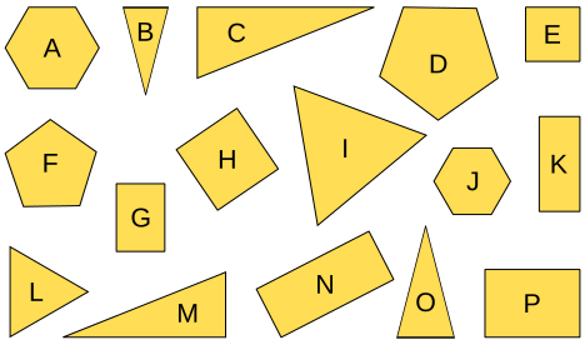
\includegraphics[scale=0.35]{matchsimilarshapes.png}
\end{minipage}
\begin{aufgabe}
	Vergleiche die obigen beiden Aufgaben. Wie würdest du in deinen eigenen Worten beschreiben, was ähnliche Figuren ausmachen?\vspace{5pt}\newline\karos{3}
\end{aufgabe}
Nachdem wir hier sehr einfache Aufgaben betrachtet haben, versuchen wir das in den nächsten beiden ein wenig anspruchsvoller und mathematischer zu betrachten.
\begin{aufgabe}
	Zeichne die folgenden Figuren $4$ mal nach. Versuche sie nun so zusammenzufügen, dass sie genauso aussieht wie die abgebildete Figur, einfach grösser.\newline
	\begin{minipage}{0.47\linewidth}
		\centering
		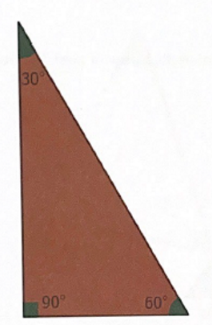
\includegraphics[scale=0.5]{30-60-90-dreieck.png}
	\end{minipage}
	\hfill
	\begin{minipage}{0.47\linewidth}
		\centering
		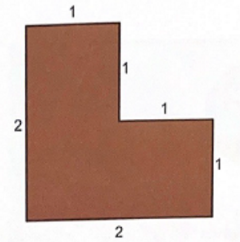
\includegraphics[scale=0.6]{l-shape.png}
	\end{minipage}
\end{aufgabe}
Wir sind also nun in der Lage, den Begriff der Ähnlichkeit auch mathematisch exakt zu definieren.
\begin{definition}
	Zwei Dreiecke heissen ähnlich, wenn sie in ihren Winkeln übereinstimmen. Das heisst, alle enthaltenen Winkel sind gleich.
	\[\alpha=\alpha',\:\beta=\beta'\text{ und } \gamma=\gamma'\]
	\begin{figure}[H]
		\centering
		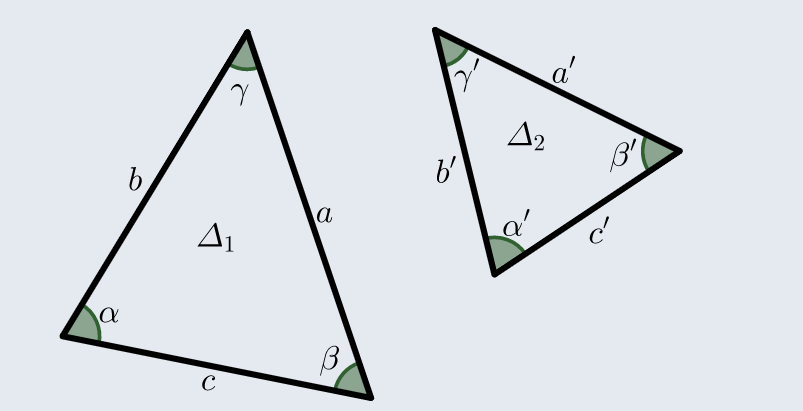
\includegraphics[scale=0.5]{ähnlichedreiecke.png}
	\end{figure}
	Um die Ähnlichkeit beider Dreiecke $\triangle_1$ und $\triangle_2$ auszudrücken, schreiben wir $\triangle_1\sim\triangle_2$.
\end{definition}
Daraus können wir auch bereits den wichtigsten Satz für ähnliche Dreiecke angeben.
\begin{satz}\label{satz:SeitenverhälnisseÄhnlichkeit}
	Falls zwei Dreiecke ähnlich sind, so sind alle einander entsprechenden Seitenverhältnisse gleich gross.
	\[\frac{a}{b}=\frac{a'}{b'}\text{ und }\frac{a}{c}=\frac{a'}{c'}\text{ und }\frac{b}{c}=\frac{b'}{c'}\]
\end{satz}
Um diesen Umstand zu beweisen, brauchen wir aber noch ein neues Werkzeug, was uns erlaubt ein geometrisches Problem in ein algebraisches, das heisst rechnerisches mit Brüchen, zu Übersetzen.
\newpage

\section{Die Strahlensätze}
Betrachten wir eine Strecke von $A$ nach $B$. Das Ziel ist, diese Strecken konstruktiv in $5$ gleich grosse Stücke zu unterteilen. Überlege dir zuerst selbstständig, wie du dies angehen würdest und tausche dich danach mit deinem Nachbarn/ deiner Nachbarin aus.
\begin{figure}[H]
	\centering
	\begin{tikzpicture}[scale=1][line cap=round,line join=round,>=triangle 45,x=1.0cm,y=1.0cm]
		\clip(-3.8,-2.5) rectangle (2.8,0.5);
		\draw [line width=1pt] (-3,0)--(2,0);
		\filldraw[black] (-3,0) circle (2pt) node[anchor=east]{$A$};
		\filldraw[black] (2,0) circle (2pt) node[anchor=west]{$B$};
	\end{tikzpicture}
\end{figure}
Betrachten wir dazu die folgende Aufgaben.
\begin{aufgabe}
	\begin{minipage}{0.57\linewidth}
		Von einem Dreieck $\triangle PQR$ ist der Umfang $U$ bekannt. Jemand möchte nun eine zu $\overline{QR}$ parallele Strecke $\overline{ST}$ anbringen, sodass $U_{\triangle PST}=\frac{1}{2}\*U_{\triangle PQR}$ ist. Wo genau muss diese Person die neue Strecke anbringen? Begründe.
	\end{minipage}
	\hfill
	\begin{minipage}{0.37\linewidth}
		\centering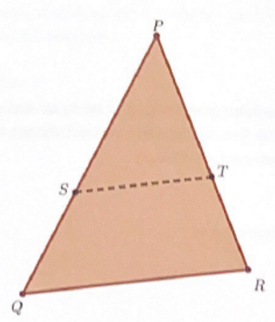
\includegraphics[scale=0.5]{einstiegstrahlensatz.png}
	\end{minipage}
	\karos{3}
\end{aufgabe}
Wir sehen also, dass wenn zwei Strahlen (in unserem Fall die Seiten $PQ$ und $PR$) von parallelen Geraden geschnitten werden, so werden die Verhältnisse der Teilstrecken vom einen Strahl auf den anderen \glqq vererbt\grqq. Diese Aussage ist auch als erster Strahlensatz bekannt.
\begin{satz}[Erster Strahlensatz]
	\begin{minipage}{0.57\linewidth}
		Gegeben seien zwei Strahlen mir einem gemeinsamen Ausgangspunkt $O$. Auf jedem Strahl liegen jeweils zwei Punkte, die wiederum von zwei Geraden verbunden werden. Betrache die Skizze rechts. Dann gilt:
		\begin{align*}
			g\parallel h&\same\frac{\overline{OA}}{\overline{OA'}}=\frac{\overline{OB}}{\overline{OB'}} && \text{1. Fassung}\\
			g\parallel h&\same\frac{\textcolor{red}{\overline{OA}}}{\textcolor{blue}{\overline{AA'}}}=\frac{\textcolor{red}{\overline{OB}}}{\textcolor{blue}{\overline{BB'}}} && \text{2. Fassung}
		\end{align*}
	\end{minipage}
	\hfill
	\begin{minipage}{0.37\linewidth}
		\centering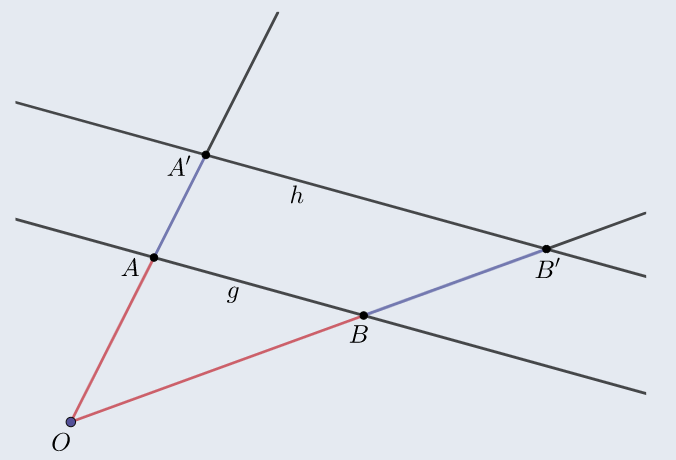
\includegraphics[scale=0.3]{ersterstrahlenssatz.png}
	\end{minipage}
\end{satz}
Dieser Satz macht eine Äquivalenzaussage. Das bedeutet, dass er in beide Richtungen verwendet werden kann. Betrachten wir dazu ein Beispiel.
\begin{beispiel}
	In der folgenden Figur sind die beiden Geraden $e$ und $f$ parallel.\vspace{5pt}\newline
	\begin{minipage}{0.57\linewidth}
		Gegeben sind folgende Strecken: $a=2$cm, $b=4$cm und $c=3$cm. Berechne die fehlende Strecke $d$.\vspace{1.5cm}\newline
		Gegeben sind folgende Strecken: $b=9$cm, $c+d=17$cm und $d=8$cm. Berechne die fehlenden Strecken $a$ und $c$.\vspace{1.5cm}
	\end{minipage}
	\hfill
	\begin{minipage}{0.37\linewidth}
		\centering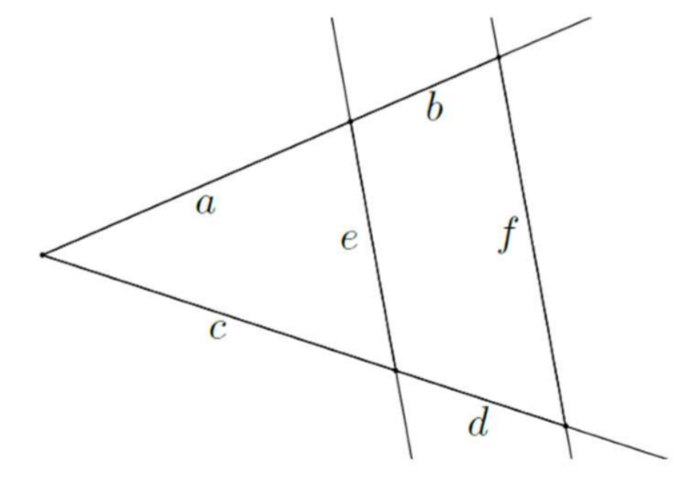
\includegraphics[scale=0.3]{strahlensatzfigur.png}
	\end{minipage}
\end{beispiel}
Der zweite Strahlensatz erlaubt uns nun noch die Länge der beiden Parallelenstrecken zu berechnen.
\begin{satz}[Zweiter Strahlensatz]
	\begin{minipage}{0.57\linewidth}
		Gegeben seien zwei Strahlen mir einem gemeinsamen Ausgangspunkt $O$. Auf jedem Strahl liegen jeweils zwei Punkte, die wiederum von zwei Geraden verbunden werden. Betrache die Skizze rechts. Dann gilt:
		\begin{align*}
			g\parallel h&\same\frac{\textcolor{red}{\overline{OA}}}{\textcolor{red}{\overline{AB}}}=\frac{\textcolor{blue}{\overline{OA'}}}{\textcolor{blue}{\overline{A'B'}}}
		\end{align*}
	\end{minipage}
	\hfill
	\begin{minipage}{0.37\linewidth}
		\centering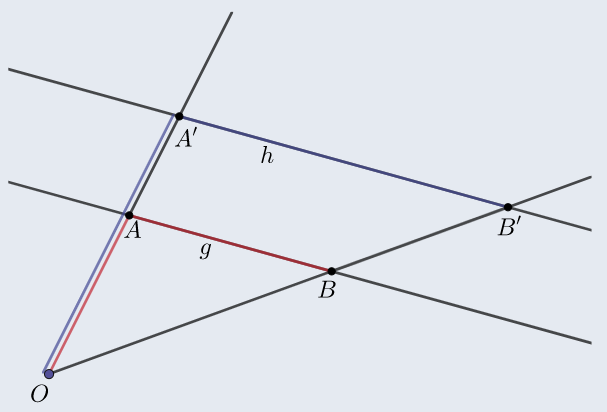
\includegraphics[scale=0.34]{zweiterstrahlensatz.png}
	\end{minipage}
\end{satz}
Betrachten wir nochmals dieselbe Figur wie oben, um ein Beispiel für den zweiten Strahlensatz zu zeigen.
\begin{beispiel}
	In der folgenden Figur sind die beiden Geraden $e$ und $f$ parallel.\vspace{5pt}\newline
	\begin{minipage}{0.57\linewidth}
		Gegeben sind folgende Strecken: $a=2$cm, $b=4$cm und $f=7$cm. Berechne die fehlende Strecke $e$.\vspace{1.5cm}\newline
		Gegeben sind folgende Strecken: $c+d=17$cm und $e=3$cm. Berechne die fehlenden Strecken $c$ und $f$.\vspace{1.5cm}
	\end{minipage}
	\hfill
	\begin{minipage}{0.37\linewidth}
		\centering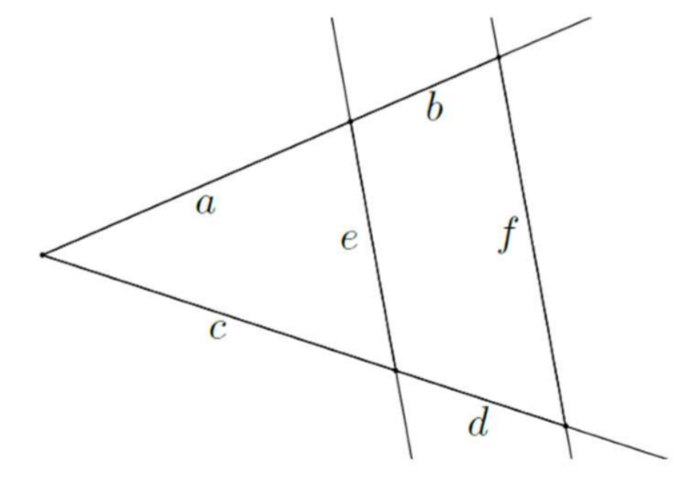
\includegraphics[scale=0.3]{strahlensatzfigur.png}
	\end{minipage}
\end{beispiel}\newpage
\begin{aufgabe}
	\begin{enumerate}
		\item In den Dreiecken sind jeweils zwei Geraden parallel. Berechne die fehlende Seite $x$.
		\begin{figure}[H]
			\centering
			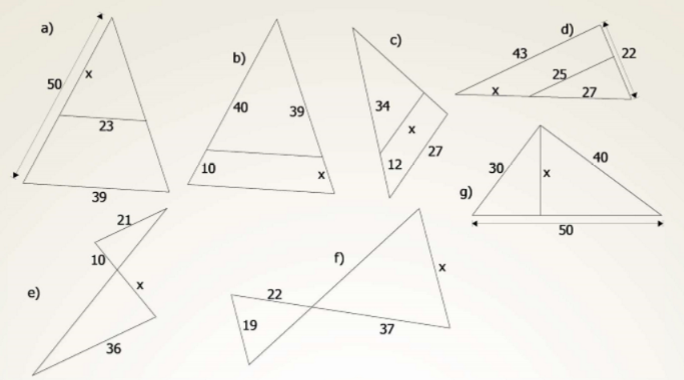
\includegraphics[scale=0.6]{aufgstrahlensatz1.png}
		\end{figure}
		\item In den Figuren gilt $g\parallel h$. Berechne die fehlenden Grössen.
		\begin{figure}[H]
			\centering
			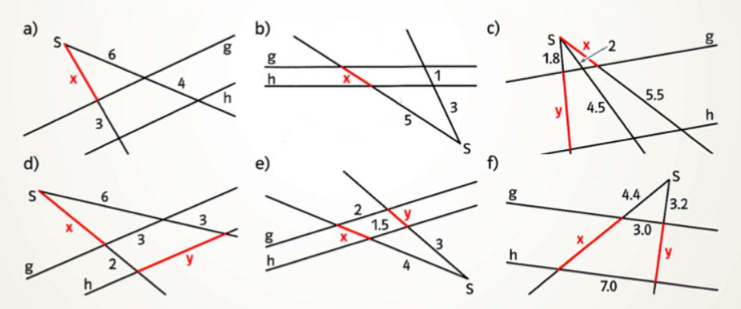
\includegraphics[scale=0.6]{aufgstrahlensatz2.png}
		\end{figure}
		\item Zwei Parallelen werden von zwei weiteren Geraden geschnitten. Berechne die fehlenden Längen.
		\begin{figure}[H]
			\centering
			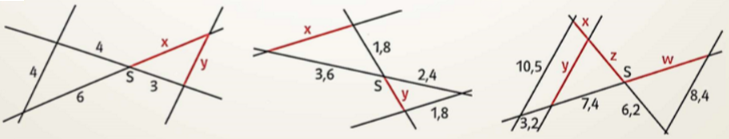
\includegraphics[scale=0.6]{aufgstrahlensatz3.png}
		\end{figure}
		\item Bestimme $s$ in der folgenden Figur auf zwei verschiedenen Wegen. Folgende Längen sind bekannt: $\overline{AB}=8$cm, $\overline{CD}=3$cm, $\overline{DA}=8$cm und $\overline{DE}=2$cm.
		\begin{figure}[H]
			\hspace{1.5cm}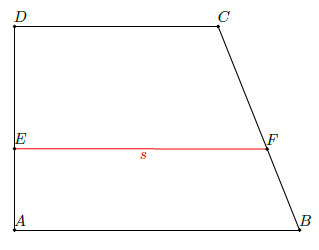
\includegraphics[scale=0.5]{aufgtrapez.png}
		\end{figure}
	\end{enumerate}
\end{aufgabe}
\section{Beweis von Satz \ref{satz:SeitenverhälnisseÄhnlichkeit}}
Wie bereits gesagt, möchten wir den Hauptsatz für ähnliche Dreiecke beweisen. Mithilfe der Strahlensätze, die wir nun kennengelernt haben, ist dies auch keine grosse Hexerei mehr. Zur Erinnerung nochmals die Behauptung:
\begin{tcolorbox}[enhanced,colback=red!5!white,fuzzy halo=2mm with gray,colframe=red!75!black]
	Falls zwei Dreiecke ähnlich sind, so sind alle einander entsprechenden Seitenverhältnisse gleich gross.
	\[\frac{a}{b}=\frac{a'}{b'}\text{ und }\frac{a}{c}=\frac{a'}{c'}\text{ und }\frac{b}{c}=\frac{b'}{c'}\]
\end{tcolorbox}
\begin{beweis}
	Betrachten wir zwei zueinander ähnliche Dreiecke $\triangle ABC$ und $\triangle A'B'C'$, die so angeordnet sind, dass die Punkte $A$ und $A'$ an derselben Stelle liegen. Dann sehen die beiden Dreiecke aufgund der Ähnlichkeit ($\alpha=\alpha'$) wie folgt aus:
	\begin{figure}[H]
		\centering
		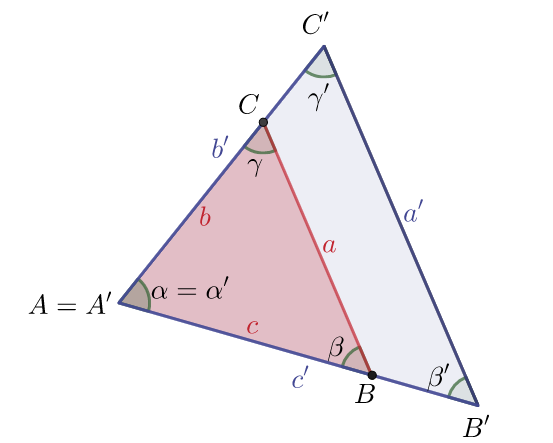
\includegraphics[scale=0.4]{beweisähnlich.png}
	\end{figure}
	Da nun auch $\beta=\beta'$ und $\gamma=\gamma'$ gilt, sind die beiden Strecken $a$ und $a'$ parallel. Das bedeutet:\vspace{5pt}\newline\karos{6}
\end{beweis}
Diese Verhältnisse können wir also genauso wie die Strahlensätze verwenden, um fehlende Strecken einer Figur zu berechnen.
\begin{aufgabe}
	\begin{enumerate}
		\item Von zwei ähnlichen Dreiecken $\triangle ABC$ und $\triangle A'B'C'$ wissen wir Folgendes: $a=9, c=8$ und $b'=c'=2$. Berechne daraus die fehlenden Seiten.
		\item In der folgenden Figur ist $M$ der Mittelpunkt der Seite $\overline{BC}$, $\overline{AB}=15$ und $\overline{AC}=25$. Welchen Flächeninhalt hat das Viereck $ABMD$.
		\begin{figure}[H]
			\hspace{1.5cm}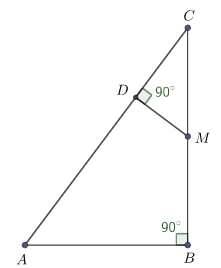
\includegraphics[scale=0.5]{aufgähnlichkeit.png}
		\end{figure}
	\end{enumerate}
\end{aufgabe}
Den Satz oben könnte man auch anders formulieren. Wie wir nämlich beim Einstieg schon festgestellt haben, sind die Seiten von ähnlichen Figuren vergrössert bzw. verkleinert. Daraus folgt also, dass es für zwei ähnliche Dreiecke eine reelle Zahl $k\in\R$ geben muss, sodass \[a'=k\*a,\quad b'=k\*b\quad\text{und}\quad c'=k\*c\]
gilt. Diese reelle Zahl $k$ wird auch als Streckfaktor bezeichnet.
\begin{definition}[Streckfaktor]
	Der \textbf{Streckfaktor} $k\in\R$ gibt das Mass einer Vergrösserung bzw. Verkleinerung an und entspricht dem Quotienten aus Bildstrecke und Ausgangsstrecke \[k=\frac{a'}{a}=\frac{b'}{b}=\frac{c'}{c}.\]
\end{definition}
Wir sehen also, das vergrösserte bzw. verkleinerte Figuren zueinander ähnlich sind. Wie verändert sich die Fläche einer vergrösserten Figur? Dazu untersuchen wir Dreiecke:
\begin{aufgabe}
	Betrachte das folgende \href{https://www.geogebra.org/m/afqa8scd}{Geogebra-Applet}. Darin sind zwei zueinander ähnliche Dreiecke abgebildet.
	\begin{enumerate}[label=\alph*)]
		\item Vergleiche die Grösse der abgebildeten Flächen und behaupte eine mathematische Formel in Abhängigkeit des Streckfaktors $k$ der Form \[A'=\gap{1.5}\*A\]
		\item Überprüfe deine Formel an unterschiedlichen Werten für $k$.
	\end{enumerate}
	\vspace{5pt}\karos{2}
	\begin{enumerate}[label=\alph*)]\setcounter{enumi}{2}
		\item Übertrage deine Behautung in den Satz \thesection.\ref{satz:VergrösserungFlächen} unten und beweise deine Behauptung auch mathematisch.
	\end{enumerate}
\end{aufgabe}
\begin{satz}\label{satz:VergrösserungFlächen}
	Bei einer Vergrösserung bzw. Verkleinerung um den Faktor $k$ gilt für den Flächeninhalt: \[A'=\gap{1.5}\*A.\]
\end{satz}
\begin{beweis}
	\textit{Tipp:} Es ist vermutlich sinnvoll, die Seiten des im Geogebra braunen Dreiecks als $a,\: b$ und $c$ zu bezeichnen und davon ausgehend die Seiten des blauen Dreiecks zu beschreiben. Im Anschluss probiere die Fläche mit diesen Seiten zu berechnen.
	\vspace{5pt}\newline\karos{5}
\end{beweis}


\newpage
\subsection*{History}
\begin{table}[H]
	\centering
	\begin{tabular}{|p{13mm}|p{20mm}|p{30mm}|p{70mm}|}\hline
		%\multicolumn{4}{|l|}{History}\\\hline
		Version & Datum & Person & Bemerkung \\\hline
		$1.0$ & 02.08.2024 & Jonas Guler & Kapitel erstellt \\\hline
		$1.1$ & 05.09.2025 & Jonas Guler & Fehler korrigiert \\\hline
		& ToDo & Jonas Guler & \\\hline
	\end{tabular}
\end{table}

\end{document}